\section{Results}
\label{sec:results}

All results in this section are from executed experiments with machine-readable artifacts
in \texttt{results/benchmark\_v2\_results.json} (and its summary
\texttt{benchmark\_v2\_summary.csv}). Every numeric value is directly traceable to these
files. The benchmark covers six encoders---five ECG foundation models (MERL, ST-MEM,
HuBERT-ECG, ECGFM-KED, ECG-FM) and a supervised S4D baseline---across four datasets, for
24 model$\times$dataset combinations. Per-class metrics are reported only for classes with
at least 10 positive and 10 negative test examples (minimum-support filtering); macro
metrics average over the qualifying classes ($k$ in Table~\ref{tab:full-benchmark}).
All headline AUROC and ECE values carry bootstrap 95\% confidence intervals (1{,}000
resamples). The reported point estimate is the full-test-set value; because the binned ECE
estimator is mildly positively biased under resampling (smaller effective bins on bootstrap
draws), the displayed ECE interval is taken to include the point estimate. One combination is
excluded: ECGFM-KED on CODE-15\% (partial architecture reconstruction, 35 missing keys,
near-chance AUROC), leaving 23 evaluated cells of the 24 model$\times$dataset combinations.

\subsection{Discrimination--Calibration Tradeoff on PTB-XL}
\label{sec:results-ptbxl}

Table~\ref{tab:full-benchmark} reports Phase~A and Phase~B results for all cells.
Figure~\ref{fig:main-heatmap} shows the Phase~A results as a heat map.

\begin{table*}[t]
\centering
\caption{Full benchmark across 6 models and 4 datasets (24 cells). AUROC and ECE shown with bootstrap 95\% CIs. ECG-FM was pretrained on MIMIC-IV-ECG ($\dagger$). Iso-ECE is macro ECE after isotonic recalibration. $k$ = number of classes meeting min-support ($\geq$10 positives and $\geq$10 negatives in the test split). Best AUROC per dataset in \textbf{bold}; best raw ECE \underline{underlined}.}
\label{tab:full-benchmark}
\small
\begin{tabular}{llcccccc}
\toprule
Dataset & Model & AUROC (95\% CI) $\uparrow$ & ECE (95\% CI) $\downarrow$ & Brier & SCE & Iso-ECE & $k$ \\
\midrule
  PTB-XL & MERL & 0.828 [0.795,0.857] & 0.087 [0.086,0.119] & 0.122 & -0.003 & 0.050 & 5 \\
   & ST-MEM & \textbf{0.838 [0.808,0.864]} & 0.124 [0.116,0.151] & 0.135 & -0.000 & 0.044 & 5 \\
   & HuBERT-ECG & 0.787 [0.749,0.824] & 0.136 [0.126,0.163] & 0.142 & -0.001 & 0.040 & 5 \\
   & ECGFM-KED & 0.769 [0.730,0.808] & 0.079 [0.079,0.112] & 0.133 & +0.007 & 0.031 & 5 \\
   & ECG-FM & 0.815 [0.778,0.848] & 0.088 [0.085,0.120] & 0.125 & +0.008 & 0.044 & 5 \\
   & S4D & 0.771 [0.738,0.805] & \underline{0.064 [0.064,0.096]} & 0.130 & +0.007 & 0.057 & 5 \\
  \midrule
  CODE-15\% & MERL & 0.865 [0.836,0.892] & 0.020 [0.019,0.027] & 0.044 & +0.002 & 0.013 & 7 \\
   & ST-MEM & \textbf{0.948 [0.938,0.956]} & 0.028 [0.025,0.033] & 0.041 & +0.000 & 0.013 & 7 \\
   & HuBERT-ECG & 0.878 [0.857,0.896] & 0.032 [0.029,0.038] & 0.046 & -0.000 & 0.014 & 7 \\
   & ECG-FM & 0.668 [0.622,0.716] & 0.024 [0.023,0.031] & 0.053 & +0.003 & 0.013 & 7 \\
   & S4D & 0.685 [0.644,0.728] & \underline{0.010 [0.010,0.017]} & 0.047 & +0.001 & 0.010 & 7 \\
  \midrule
  CPSC2018 & MERL & 0.910 [0.896,0.921] & 0.024 [0.024,0.034] & 0.048 & -0.001 & 0.019 & 9 \\
   & ST-MEM & \textbf{0.950 [0.940,0.958]} & 0.034 [0.033,0.041] & 0.042 & +0.001 & 0.016 & 9 \\
   & HuBERT-ECG & 0.876 [0.862,0.889] & 0.051 [0.049,0.060] & 0.068 & +0.004 & 0.020 & 9 \\
   & ECGFM-KED & 0.821 [0.805,0.838] & 0.025 [0.025,0.037] & 0.072 & +0.002 & 0.021 & 9 \\
   & ECG-FM & 0.847 [0.832,0.861] & 0.032 [0.032,0.043] & 0.067 & +0.002 & 0.021 & 9 \\
   & S4D & 0.803 [0.784,0.823] & \underline{0.023 [0.023,0.034]} & 0.075 & +0.000 & 0.021 & 9 \\
  \midrule
  MIMIC-IV-ECG & MERL & \textbf{0.861 [0.827,0.892]} & 0.074 [0.066,0.094] & 0.082 & -0.005 & 0.044 & 5 \\
   & ST-MEM & 0.854 [0.816,0.890] & 0.080 [0.072,0.098] & 0.082 & -0.010 & 0.037 & 5 \\
   & HuBERT-ECG & 0.795 [0.758,0.829] & 0.106 [0.098,0.128] & 0.113 & -0.015 & 0.043 & 5 \\
   & ECGFM-KED & 0.732 [0.689,0.770] & 0.063 [0.059,0.086] & 0.097 & -0.004 & 0.058 & 5 \\
   & ECG-FM$^\dagger$ & 0.771 [0.734,0.813] & 0.076 [0.072,0.101] & 0.097 & -0.001 & 0.036 & 5 \\
   & S4D & 0.793 [0.758,0.826] & \underline{0.043 [0.043,0.067]} & 0.087 & -0.004 & 0.040 & 5 \\
\bottomrule
\end{tabular}
\end{table*}

\begin{figure}[t]
  \centering
  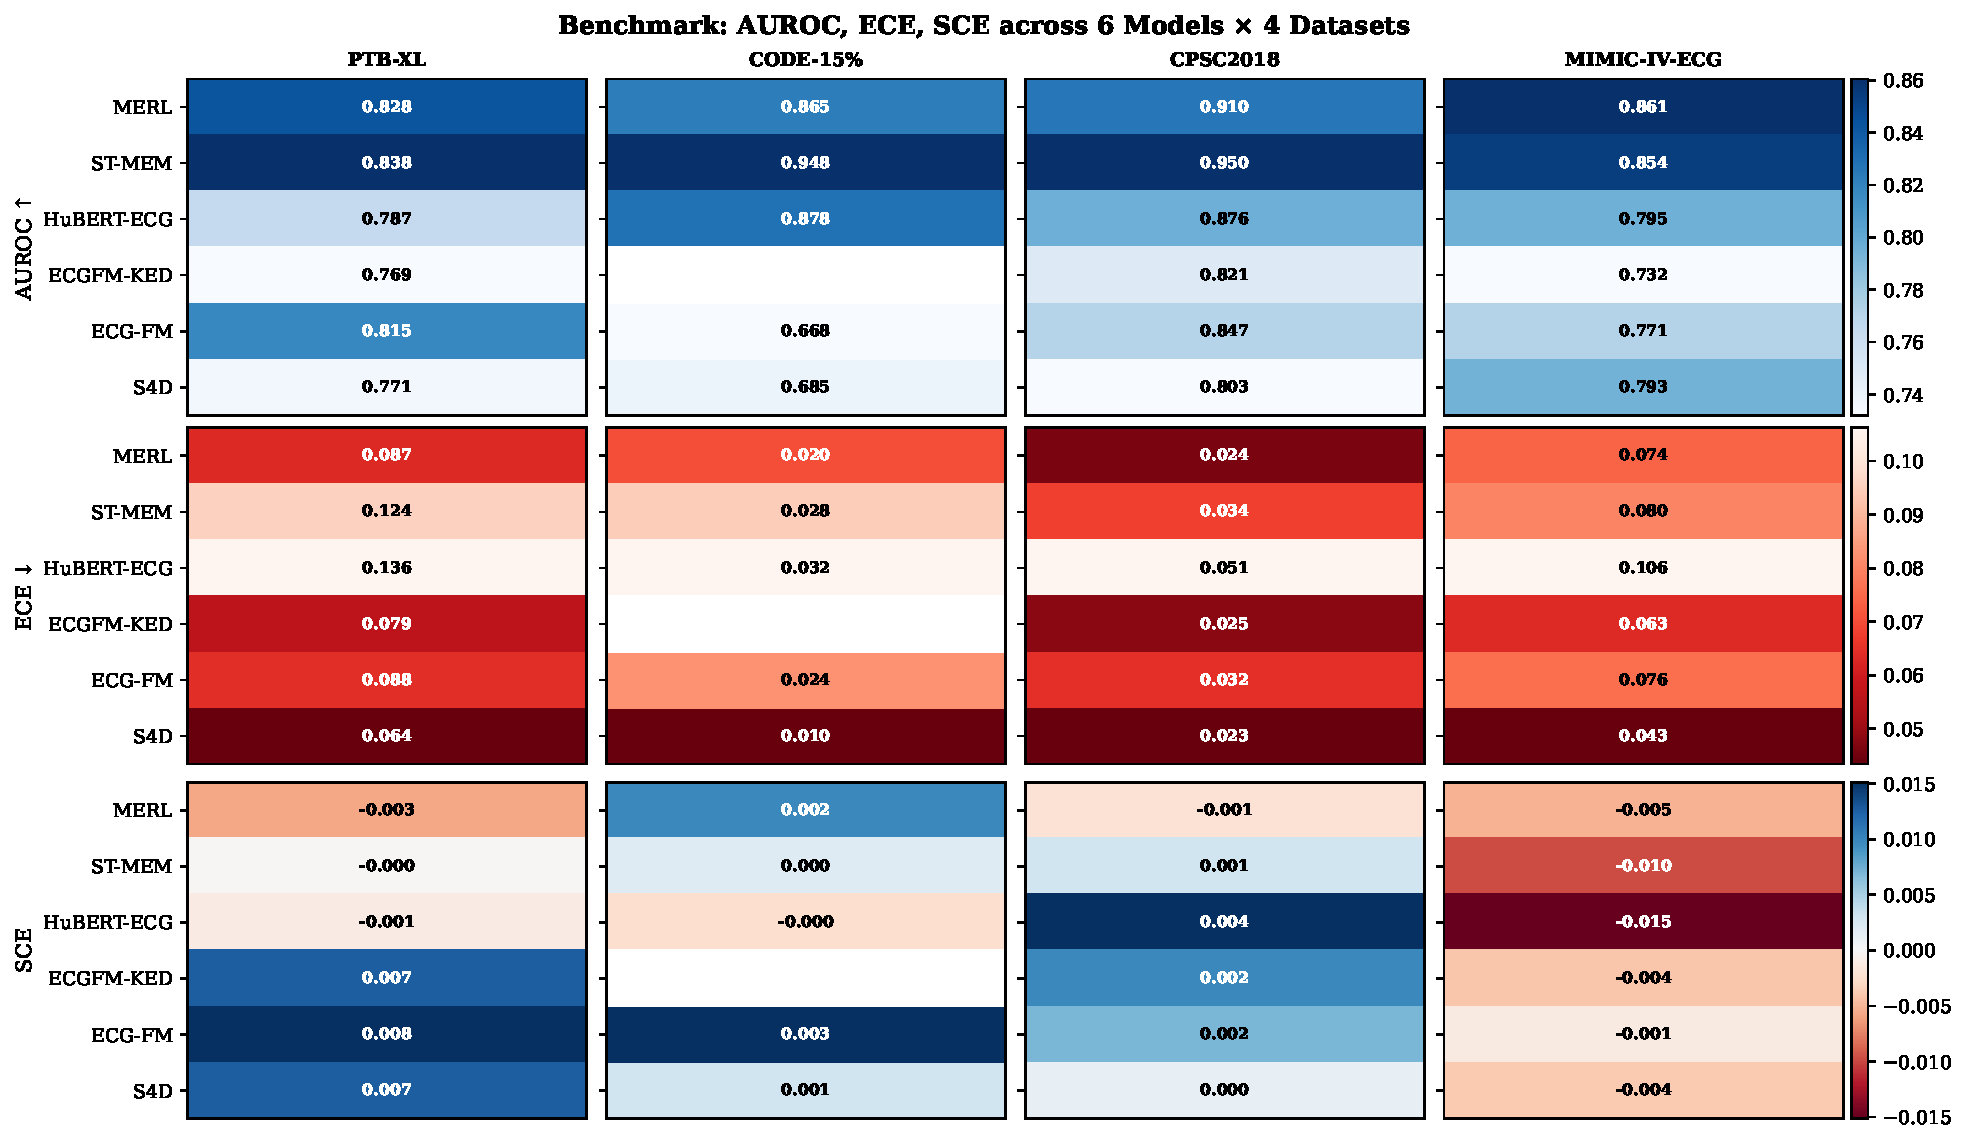
\includegraphics[width=0.98\linewidth]{figures/fig1_main_results_heatmap.pdf}
  \caption{Phase A results across all six models and four datasets.
    Top: AUROC. Middle: ECE. Bottom: SCE. All values are from executed experiments
    with patient-level splits. The ECGFM-KED $\times$ CODE-15\% cell is blank (excluded).}
  \label{fig:main-heatmap}
\end{figure}

On PTB-XL (5-class multi-label rhythm), ST-MEM achieves the highest AUROC (0.838) but poor
calibration (ECE 0.124), and the masked-prediction model HuBERT-ECG is the worst calibrated
overall (ECE 0.136) while ranking mid-pack on discrimination (AUROC 0.787). The supervised
S4D baseline achieves the best calibration (ECE 0.064) despite the lowest AUROC (0.771).
All five foundation models exceed S4D's ECE by 0.015 (ECGFM-KED) to 0.072 (HuBERT-ECG),
creating a discrimination--calibration tradeoff that is invisible to AUROC-only reporting.
Figure~\ref{fig:tradeoff} visualises this tradeoff across all four datasets, and
Figure~\ref{fig:reliability-ptbxl} shows the corresponding reliability diagrams.

\begin{figure}[t]
  \centering
  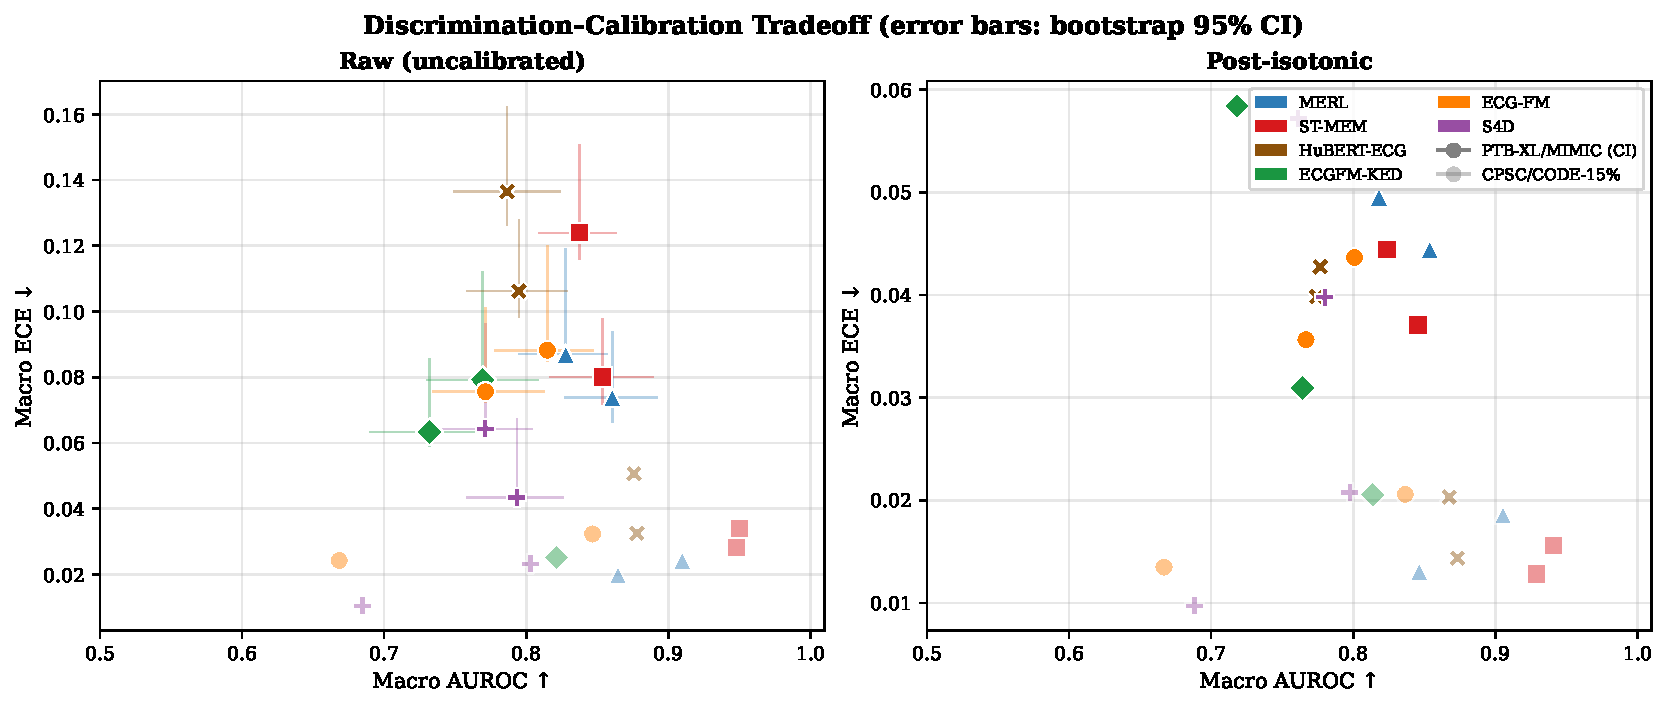
\includegraphics[width=0.96\linewidth]{figures/fig2_tradeoff_scatter.pdf}
  \caption{Discrimination--calibration tradeoff (error bars: bootstrap 95\% CIs on the
    multi-morbidity datasets). Left: raw probabilities; on PTB-XL and MIMIC-IV-ECG,
    higher-AUROC models tend to have higher ECE. Right: after isotonic recalibration, the
    vertical spread collapses. Colour encodes model; marker encodes pretraining objective.}
  \label{fig:tradeoff}
\end{figure}

\begin{figure}[t]
  \centering
  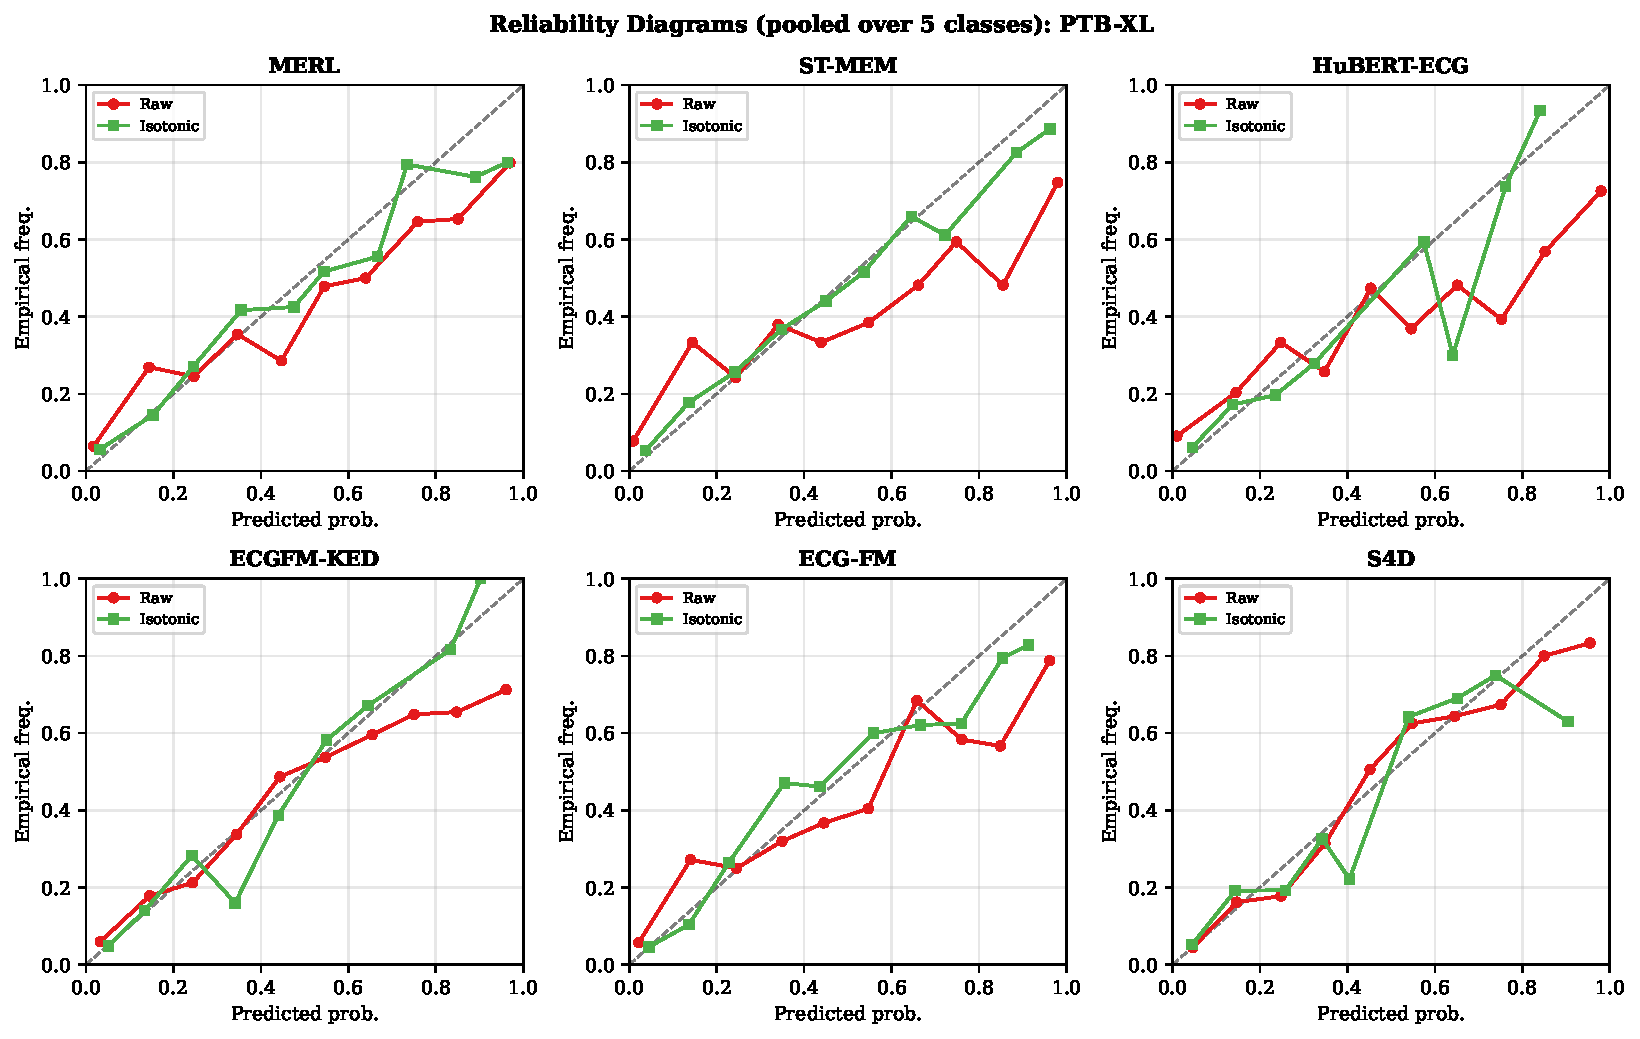
\includegraphics[width=0.98\linewidth]{figures/fig_reliability_D1.pdf}
  \caption{Reliability diagrams on PTB-XL (pooled over the five superclasses), raw vs.\
    isotonic. ST-MEM and HuBERT-ECG deviate most from the diagonal before recalibration;
    isotonic regression restores near-diagonal reliability for all encoders.}
  \label{fig:reliability-ptbxl}
\end{figure}

\subsection{Disappearance of the Tradeoff: CPSC2018, CODE-15\%, and MIMIC-IV-ECG}
\label{sec:results-cpsc}

The tradeoff vanishes on the single-label arrhythmia datasets. On CPSC2018, ST-MEM achieves
both the highest AUROC (0.950) and a low ECE (0.034); S4D achieves the lowest ECE (0.023).
Every model is well-calibrated (ECE 0.023--0.051, the maximum being HuBERT-ECG). The pattern
is consistent across all six encoders.

We attribute this disappearance to task structure. PTB-XL is a multi-label rhythm
classification task with five correlated superclasses (NORM, MI, STTC, CD, HYP); the linear
probe must simultaneously output valid probabilities for correlated, partially overlapping
classes. CPSC2018, CODE-15\%, and MIMIC-IV-ECG are effectively single-label (or
low-co-occurrence) tasks with cleaner class boundaries. The multi-label structure creates
geometrically harder representation-to-probability mappings, where the probe must apportion
probability mass across correlated outputs simultaneously.

\paragraph{CODE-15\% (expanded sample).}
At the original 2{,}000-record/part-0 subset, CODE-15\%'s rare arrhythmia classes
(prevalence 1.6--2.8\%) did not clear the minimum-support threshold, leaving only one
evaluable class. We therefore expanded CODE-15\% to ${\sim}8{,}000$ records sampled across
HDF5 parts 0--4, after which all seven classes (the six arrhythmias plus a normal-ECG
reference) qualify. On this powered sample, ST-MEM dominates (AUROC 0.948, ECE 0.028),
followed by HuBERT-ECG (0.878) and MERL (0.865); ECG-FM (0.668) and S4D (0.685) trail.
Every encoder is well-calibrated (ECE 0.010--0.032), with S4D best (0.010). ECGFM-KED is
excluded here owing to its partial architecture reconstruction.

\paragraph{MIMIC-IV-ECG.}
Figure~\ref{fig:mimic-indomain} reports results on MIMIC-IV-ECG (800{,}035 available
records; 2{,}000 sampled at natural prevalence). Labels for six conditions are parsed from
the machine-measurement reports; we apply the same minimum-support filter, which retains
five classes (sinus rhythm, AF, RBBB, LVH, myocardial infarction) and excludes LBBB (9 test
positives); per-class support is given in Table~\ref{tab:mimic-support}. All encoders are
reasonably calibrated (ECE 0.043--0.106). MERL attains the best discrimination (AUROC 0.861),
narrowly ahead of ST-MEM (0.854); S4D is best calibrated (ECE 0.043). Per class, ST-MEM
reaches AUROC 0.96 for AF and 0.95 for RBBB but only 0.77 for myocardial infarction and 0.74
for LVH---the clinically hardest endpoints. Reliability diagrams are shown in
Figure~\ref{fig:reliability-mimic}.

\begin{figure}[t]
  \centering
  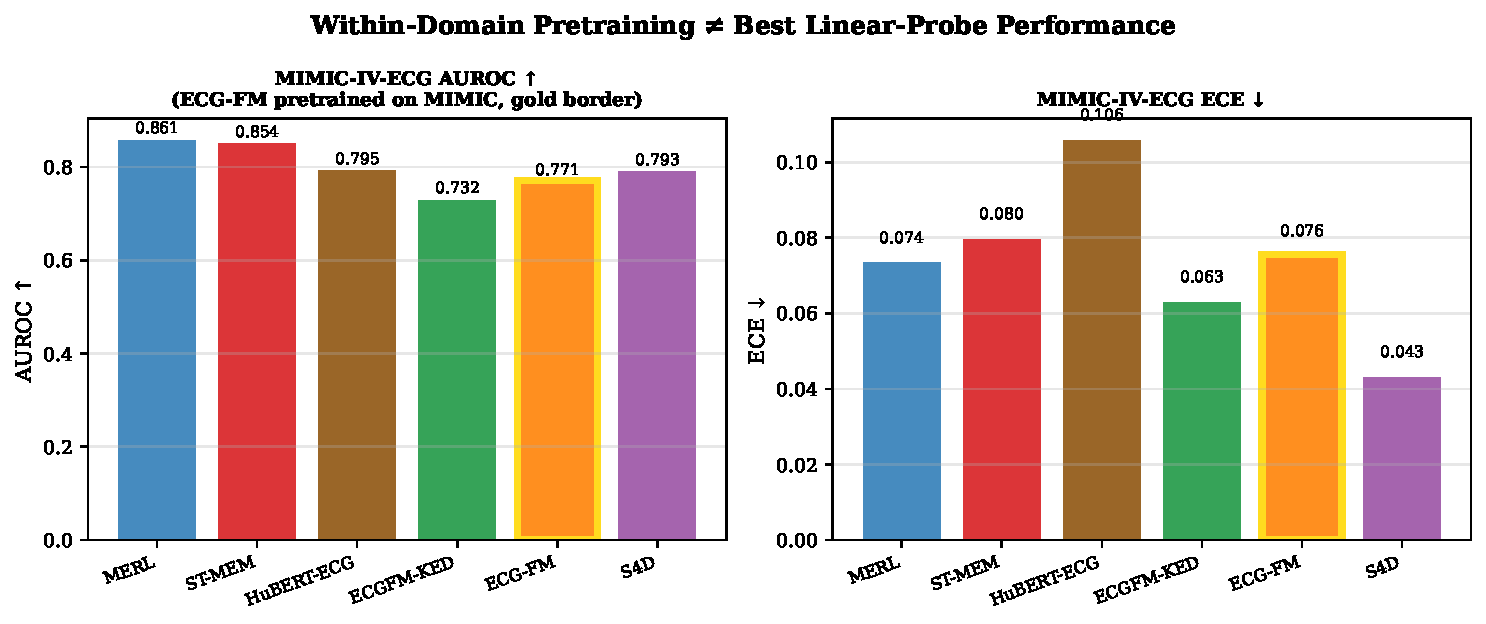
\includegraphics[width=0.90\linewidth]{figures/fig_mimic_indomain.pdf}
  \caption{MIMIC-IV-ECG benchmark results. Left: AUROC. Right: ECE. ECG-FM (gold border)
    was pretrained on MIMIC-IV-ECG yet achieves only AUROC 0.771, behind MERL (0.861),
    ST-MEM (0.854), and even the supervised S4D baseline (0.793). Within-domain pretraining
    of the \emph{backbone} does not guarantee superior linear-probe performance.}
  \label{fig:mimic-indomain}
\end{figure}

\begin{figure}[t]
  \centering
  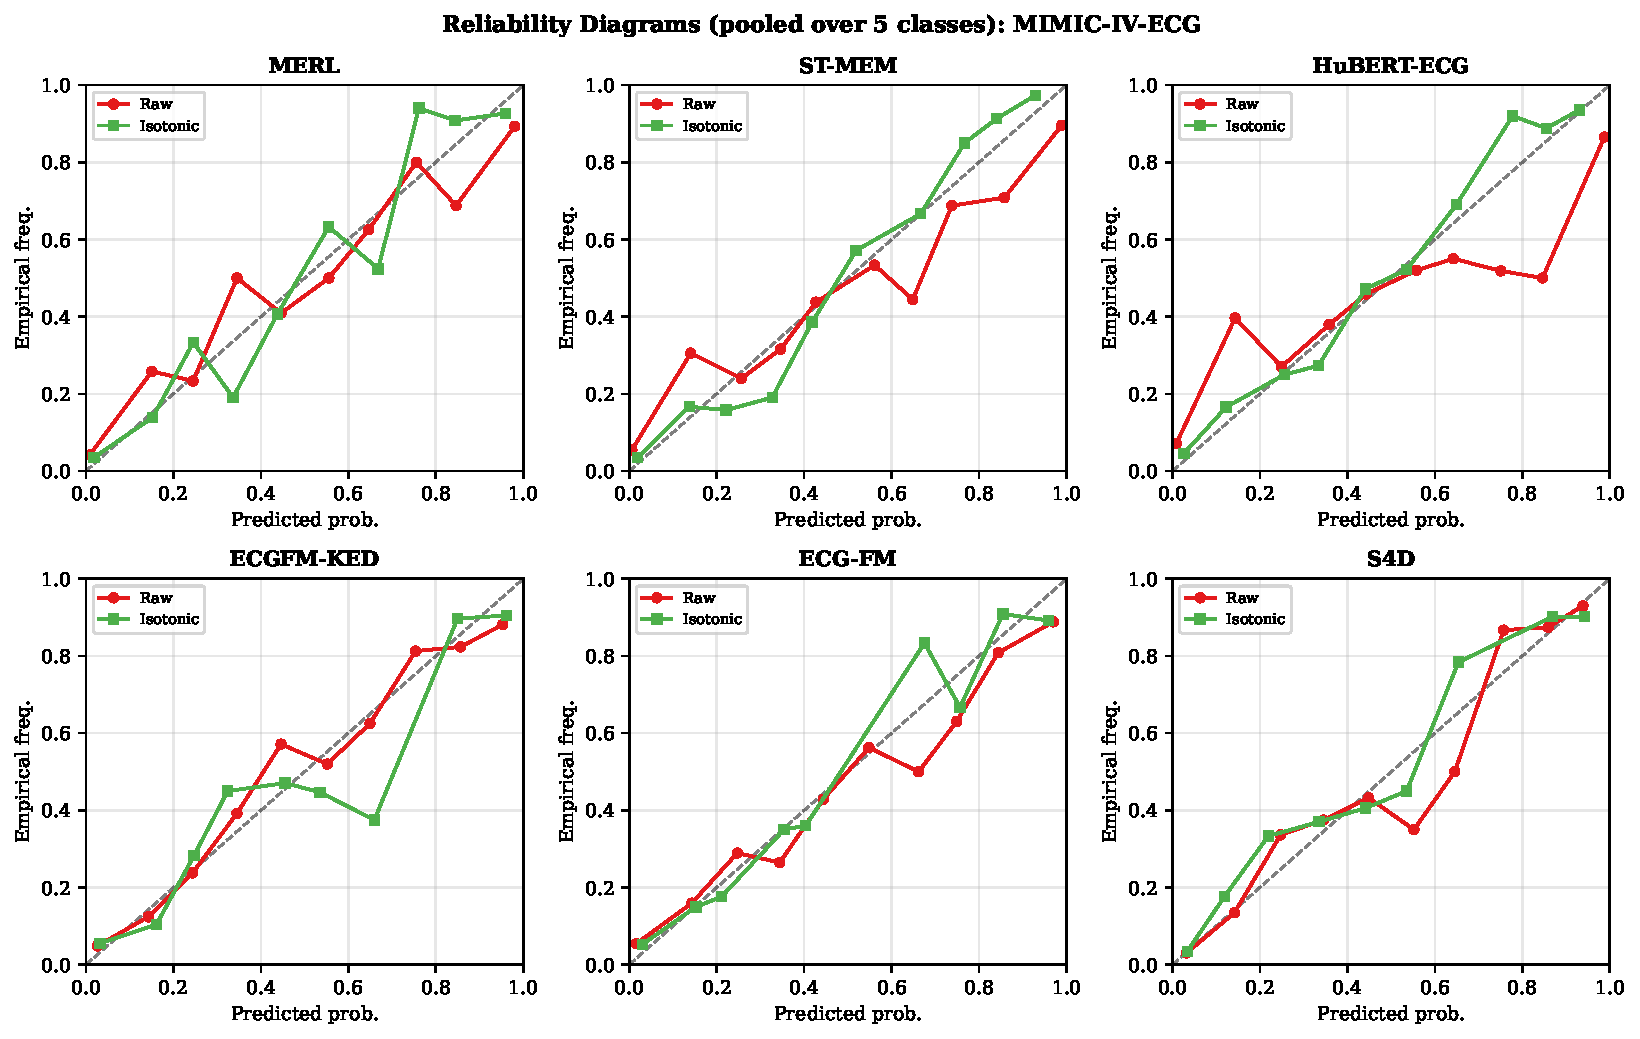
\includegraphics[width=0.98\linewidth]{figures/fig_reliability_D5.pdf}
  \caption{Reliability diagrams on MIMIC-IV-ECG (pooled over the five qualifying classes),
    raw vs.\ isotonic. HuBERT-ECG is the most miscalibrated; isotonic recalibration improves
    all encoders.}
  \label{fig:reliability-mimic}
\end{figure}

\begin{table}[t]
\centering
\caption{MIMIC-IV-ECG per-class support (2{,}000 records, natural prevalence from machine-measurement reports). Classes with $\geq$10 positives and $\geq$10 negatives in the test split are included in macro metrics.}
\label{tab:mimic-support}
\small
\begin{tabular}{lccc}
\toprule
Class & Test positives & Test negatives & Included \\
\midrule
  Sinus rhythm & 269 & 32 & \checkmark \\
  Atrial fibrillation & 40 & 261 & \checkmark \\
  RBBB & 28 & 273 & \checkmark \\
  LBBB & 9 & 292 & -- \\
  LVH & 22 & 279 & \checkmark \\
  Myocardial infarction & 62 & 239 & \checkmark \\
\bottomrule
\end{tabular}
\end{table}

A striking within-domain finding: despite ECG-FM being \emph{pretrained on MIMIC-IV-ECG},
it achieves only AUROC 0.771, behind MERL ($+0.090$) and ST-MEM ($+0.083$) in every resplit,
and statistically tied with the supervised S4D baseline ($+0.022$, not robust across seeds;
Section~\ref{sec:extended-robustness}). We attribute this to the frozen linear-probe protocol:
ECG-FM's hybrid contrastive+generative objective may encode features useful for
self-supervised tasks on MIMIC but not optimally linearly separable for the
machine-measurement classification targets. This is a concrete example of why pretraining
domain alignment is necessary but not sufficient for downstream discrimination and
calibration quality.

\subsection{Pretraining Objective and Calibration Direction}
\label{sec:results-pretrain}

Figure~\ref{fig:sce} shows signed calibration error by model and dataset.

\begin{figure}[t]
  \centering
  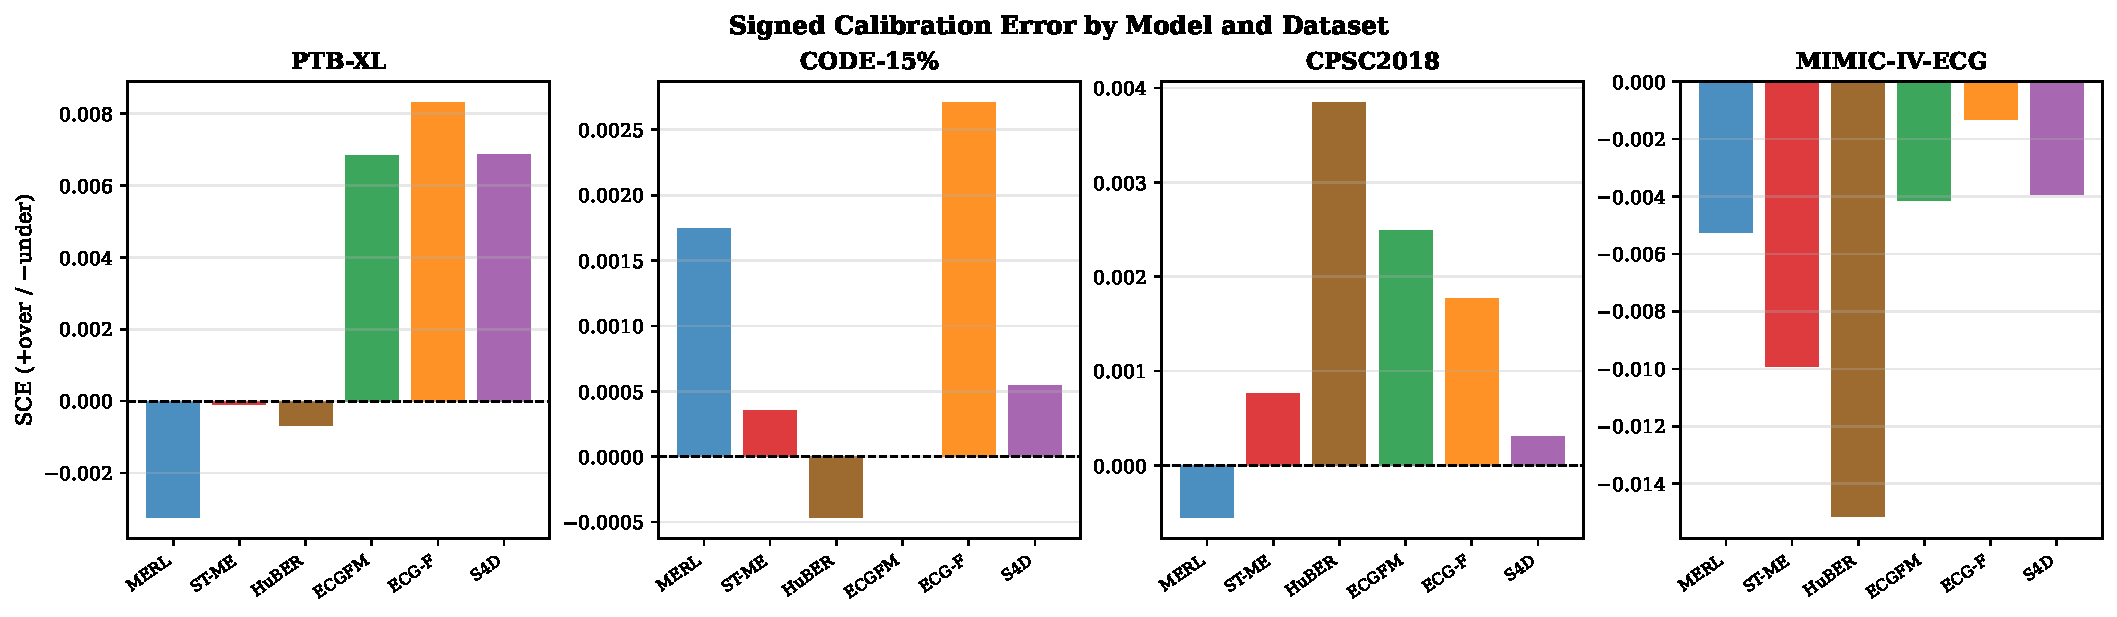
\includegraphics[width=0.95\linewidth]{figures/fig4_sce_analysis.pdf}
  \caption{Signed calibration error by model and dataset. On PTB-XL, MERL (contrastive)
    shows the strongest underconfidence ($-0.003$); the masked-prediction models (ST-MEM,
    HuBERT-ECG) are near-neutral; and knowledge-enhanced, hybrid, and supervised models are
    mildly overconfident.}
  \label{fig:sce}
\end{figure}

A graded, objective-dependent signature emerges on PTB-XL. MERL (contrastive InfoNCE) shows
the strongest underconfidence ($\text{SCE}=-0.003$), consistent with Hekler et
al.~\citep{hekler2025beyond}, who report that contrastively pretrained vision FMs are
underconfident in-distribution. The two masked-prediction models are near-neutral
(ST-MEM $\text{SCE}=-0.0001$, HuBERT-ECG $-0.0007$), while the knowledge-enhanced
(ECGFM-KED, $+0.007$), hybrid (ECG-FM, $+0.008$), and supervised (S4D, $+0.007$) models are
mildly overconfident.

Feature geometry (Figure~\ref{fig:feature-geometry}) provides a mechanistic view. MERL's
contrastive objective produces extreme feature spread (std of L2 norms 34.8) versus 0.23
(ST-MEM), 0.63 (HuBERT-ECG), 0.12 (ECGFM-KED), and 0.75 (ECG-FM); this norm-uniform
representation space yields diffuse, underconfident probabilities under a linear probe.
Separately, the \emph{unsigned} calibration error tracks class separation rather than sign:
HuBERT-ECG has the highest cosine class separation (0.046) and the highest ECE (0.136), and
ST-MEM the second highest separation (0.017) and second-highest ECE---high separation
concentrates predictions near 0/1, enlarging per-bin gaps even when the signed bias cancels.

\begin{figure}[t]
  \centering
  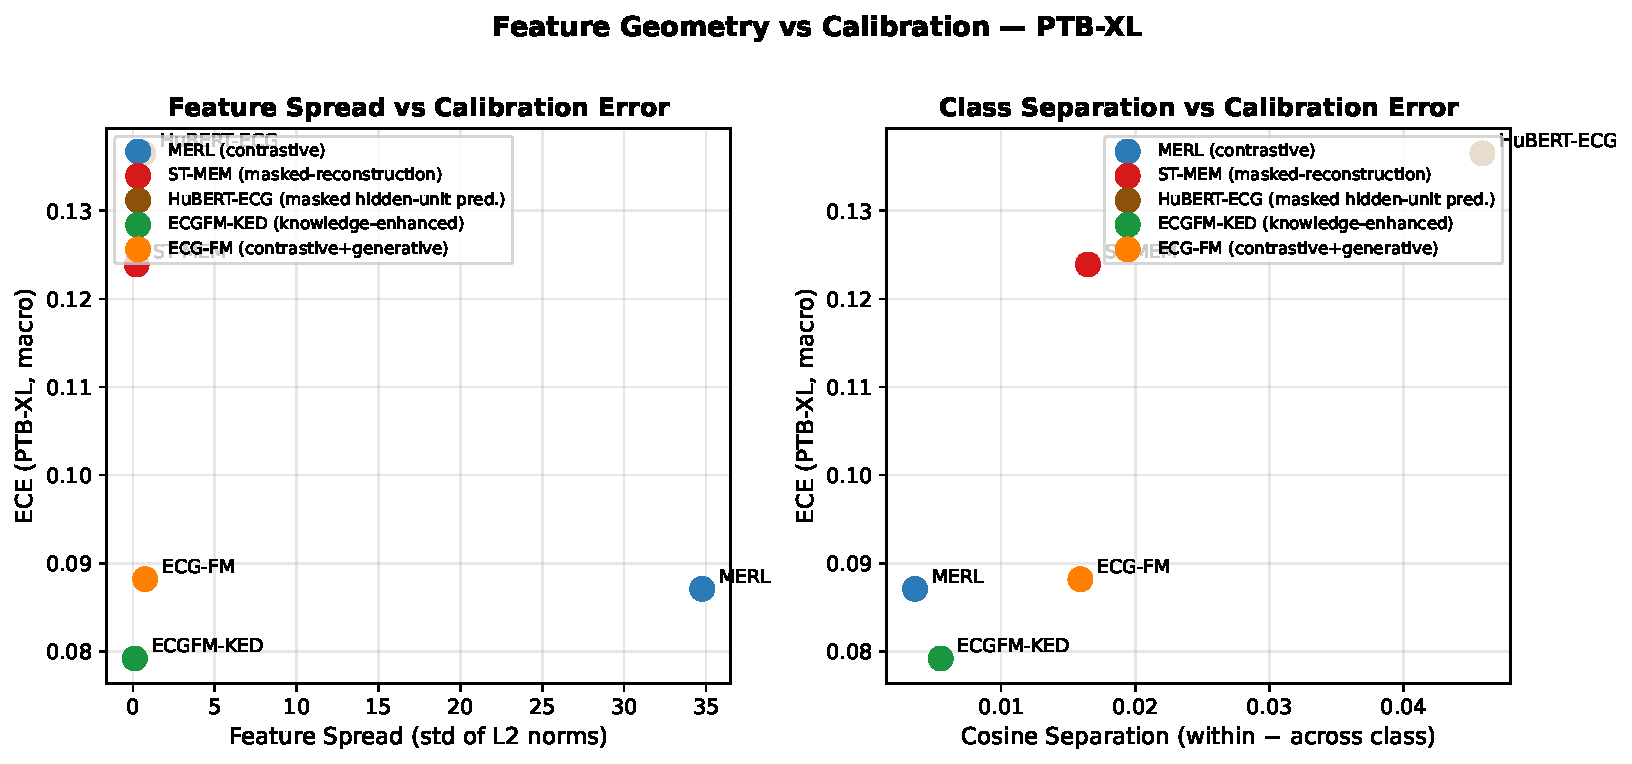
\includegraphics[width=0.95\linewidth]{figures/fig6_feature_geometry.pdf}
  \caption{Feature geometry vs.\ calibration error on PTB-XL (5 FMs). Left: feature spread
    (std of L2 norms) vs.\ ECE---MERL's extreme spread accompanies its underconfidence.
    Right: cosine class separation vs.\ ECE---HuBERT-ECG has the highest separation and the
    highest ECE. Computed on the 2{,}000-record PTB-XL sample with seed 42.}
  \label{fig:feature-geometry}
\end{figure}

\subsection{Pareto Frontier and Composite Model Selection}
\label{sec:results-pareto}

Figure~\ref{fig:pareto} shows the AUROC--ECE Pareto frontier per dataset, with the composite
score $C(\alpha)=\alpha\,\text{AUROC}+(1-\alpha)(1-\text{ECE}/\text{ECE}_{\max})$.

\begin{figure}[t]
  \centering
  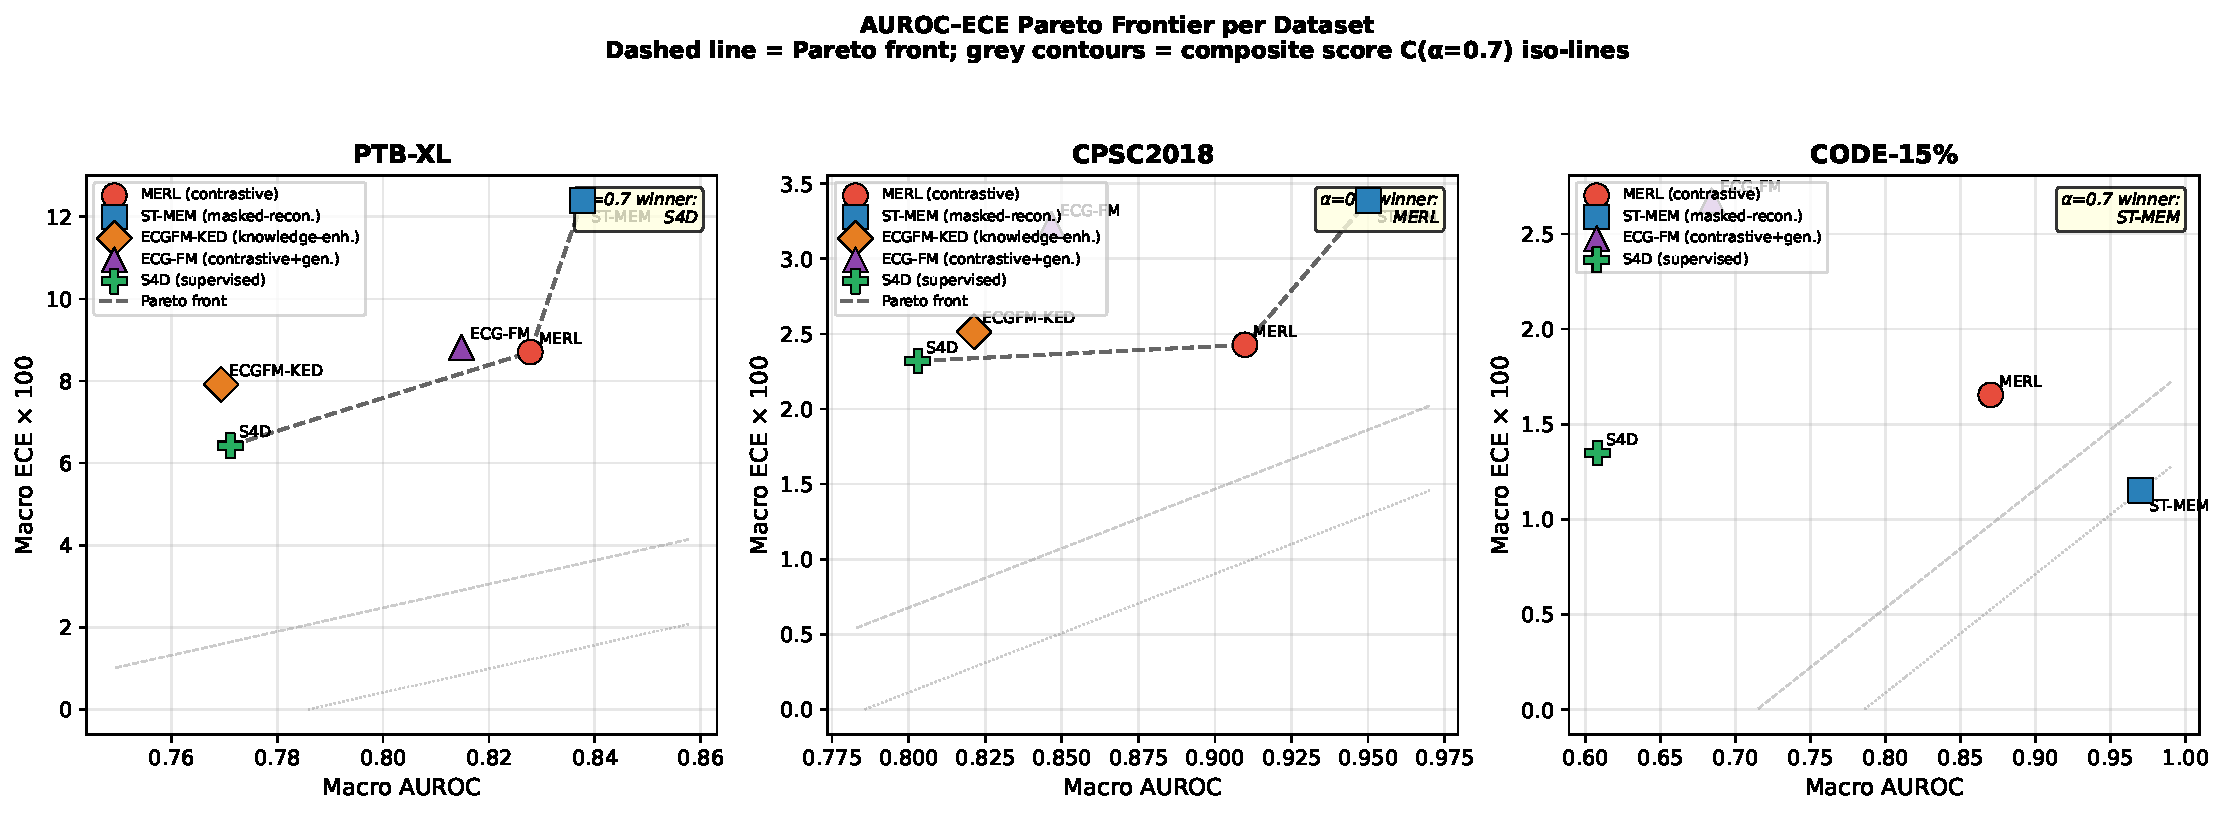
\includegraphics[width=0.98\linewidth]{figures/fig7_pareto_frontier.pdf}
  \caption{AUROC--ECE Pareto frontier per dataset. Dashed lines connect Pareto-optimal
    models; grey contours are $C(\alpha=0.7)$ iso-lines. MERL, ST-MEM, and S4D recur on the
    frontier; no single model dominates both dimensions on PTB-XL.}
  \label{fig:pareto}
\end{figure}

On PTB-XL, MERL, ST-MEM, and S4D form the Pareto-optimal set; no model dominates both axes.
The composite winner depends on $\alpha$: at $\alpha=0.7$, \textbf{S4D ranks first} (0.699),
while ST-MEM---the AUROC leader---falls to 5th of 6 (0.614) and HuBERT-ECG ranks last
(0.551); at $\alpha=0.9$ (discrimination-dominated), MERL wins (0.781). Crucially, the
ordering \emph{inverts} after isotonic recalibration: ST-MEM rises to first at $\alpha=0.7$
($C=0.789$) because its high AUROC is now paired with a low post-hoc ECE. Thus the recommended
model depends jointly on the practitioner's calibration--discrimination preference and on
whether recalibration is applied. On CPSC2018, CODE-15\%, and MIMIC-IV-ECG, MERL, ST-MEM, and
S4D recur on the Pareto front, with ST-MEM winning the discrimination-dominated regime
($\alpha=0.9$) on the two large arrhythmia datasets.

\subsection{Recalibration Comparison}
\label{sec:results-recalib}

Figures~\ref{fig:recal} and~\ref{fig:ece-reduction} compare ECE before and after
recalibration.

\begin{figure}[t]
  \centering
  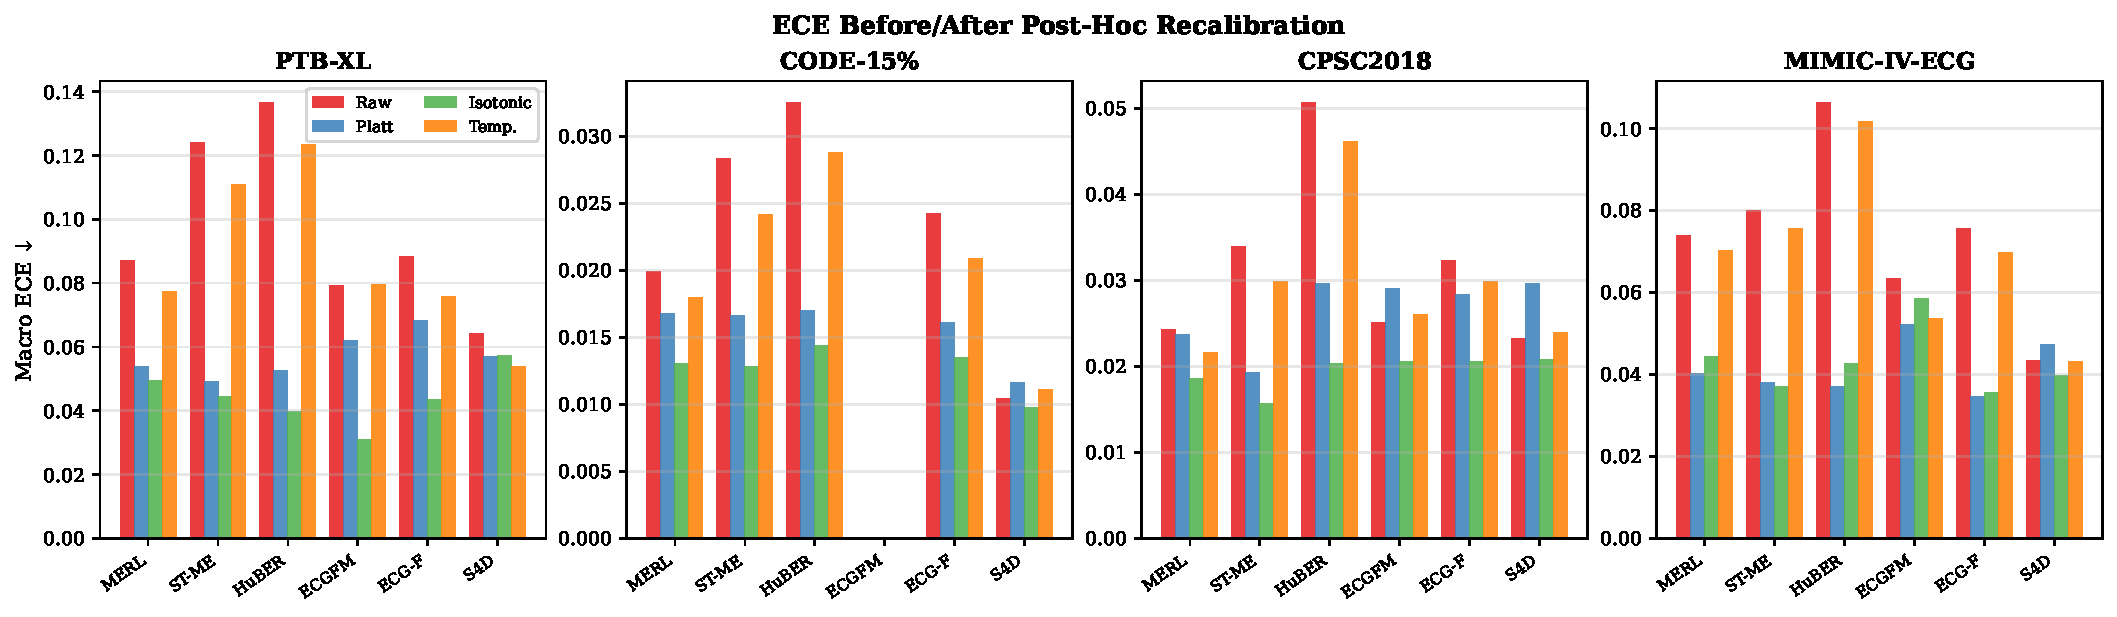
\includegraphics[width=0.98\linewidth]{figures/fig3_recalibration_comparison.pdf}
  \caption{ECE before recalibration and after Platt, isotonic, and temperature scaling for
    each model $\times$ dataset. Isotonic consistently achieves the lowest ECE on PTB-XL and
    MIMIC-IV-ECG. Platt and temperature scaling preserve AUROC by construction.}
  \label{fig:recal}
\end{figure}

\begin{figure}[t]
  \centering
  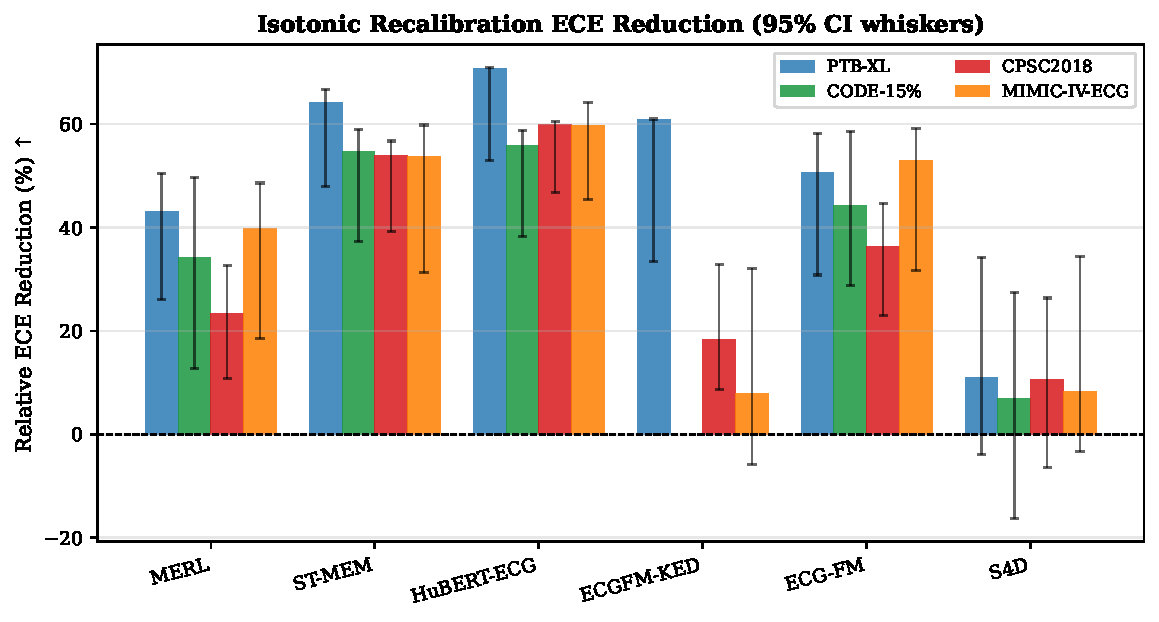
\includegraphics[width=0.95\linewidth]{figures/fig5_ece_reduction.pdf}
  \caption{Relative ECE reduction after isotonic recalibration
    $\bigl((\mathrm{ECE}_\mathrm{raw}-\mathrm{ECE}_\mathrm{iso})/\mathrm{ECE}_\mathrm{raw}\bigr)$,
    with bootstrap 95\% CI whiskers. Isotonic reduces PTB-XL ECE by 43--71\% across the
    foundation models.}
  \label{fig:ece-reduction}
\end{figure}

\paragraph{PTB-XL.}
Isotonic regression reduces foundation-model ECE by 43--71\%:
HuBERT-ECG $0.136\!\to\!0.040$ ($-71\%$);
ST-MEM $0.124\!\to\!0.044$ ($-64\%$);
ECGFM-KED $0.079\!\to\!0.031$ ($-61\%$);
ECG-FM $0.088\!\to\!0.044$ ($-51\%$);
MERL $0.087\!\to\!0.050$ ($-43\%$).
The already-well-calibrated S4D improves least ($0.064\!\to\!0.057$, $-11\%$, CI includes 0).
AUROC reductions are modest (0.5--1.7\%). Platt scaling reduces ECE by 14--38\% while fully
preserving AUROC.

\paragraph{CPSC2018, CODE-15\%, and MIMIC-IV-ECG.}
Recalibration improves already-low ECE by smaller margins. On CPSC2018, isotonic roughly
halves ST-MEM's ECE ($0.034\!\to\!0.016$). On CODE-15\%, encoders are near-calibrated and
isotonic changes are small (e.g., ST-MEM $0.028\!\to\!0.013$). On MIMIC-IV-ECG, isotonic
brings every encoder to ECE 0.036--0.058 (ST-MEM $0.080\!\to\!0.037$; ECG-FM
$0.076\!\to\!0.036$).

\subsection{Calibration-Set Size Efficiency}
\label{sec:results-calsize}

Figure~\ref{fig:calsize} shows ECE vs.\ calibration-set size for ST-MEM on PTB-XL.

\begin{figure}[t]
  \centering
  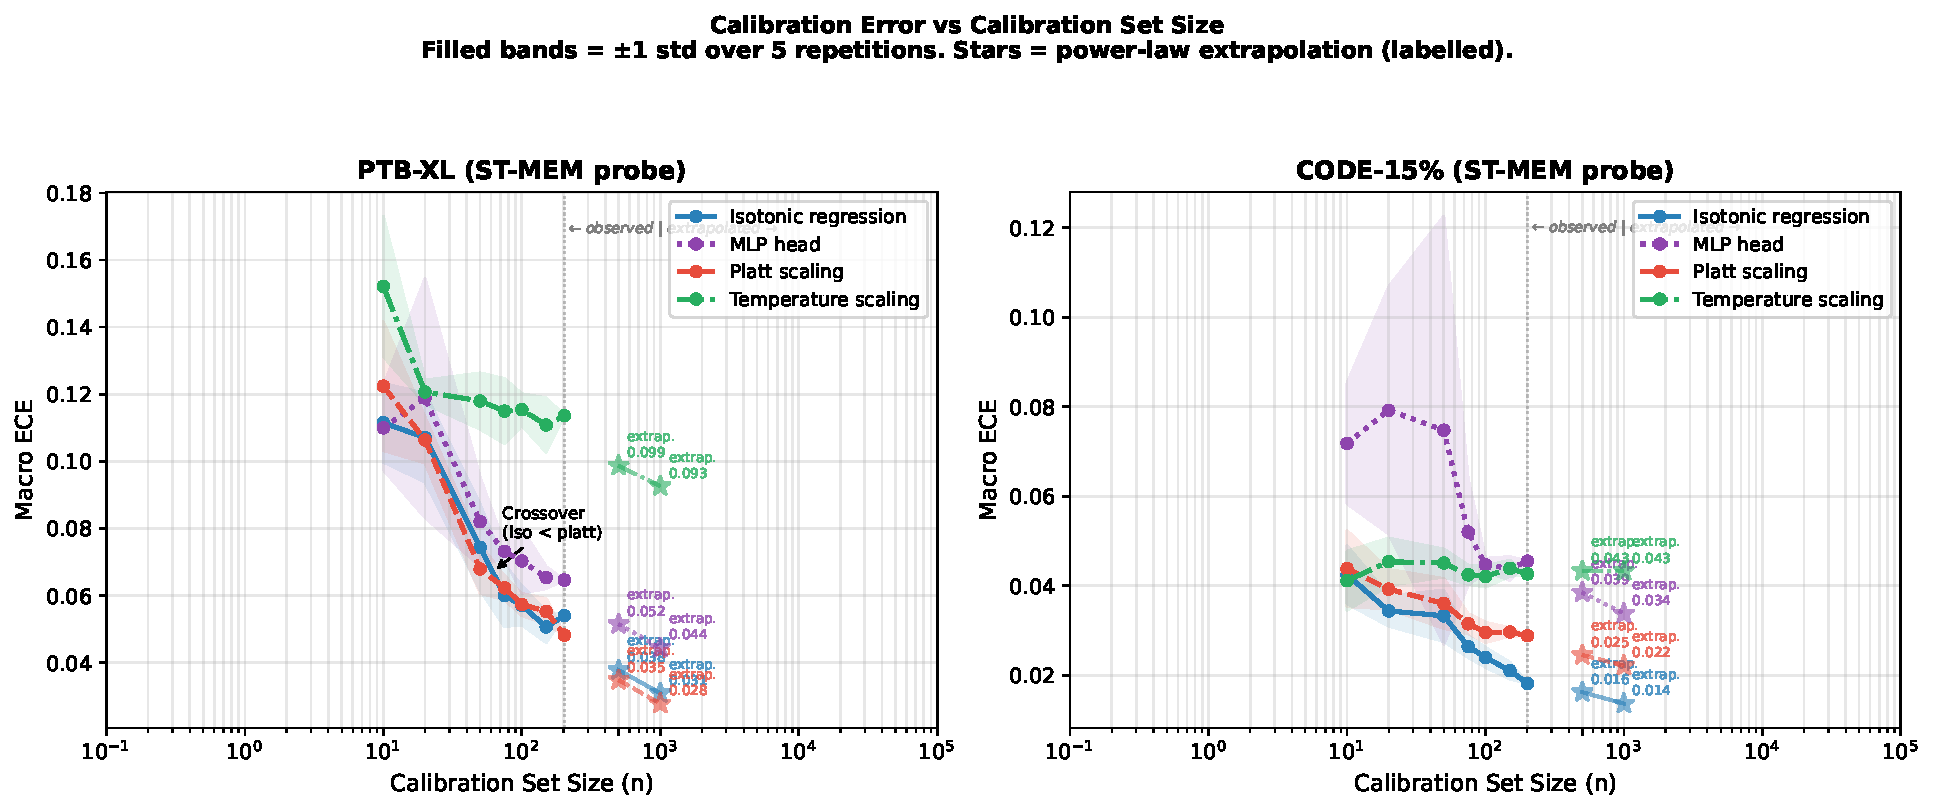
\includegraphics[width=0.98\linewidth]{figures/fig10_calsize_curves.pdf}
  \caption{ECE vs.\ calibration set size $n$. Filled bands show $\pm$1 std over 5 repetitions.
    Stars denote power-law extrapolations (``extrap.''). On PTB-XL, isotonic regression
    overtakes Platt scaling at approximately $n=63$; below this threshold Platt scaling is
    preferred. Extrapolations suggest isotonic ECE${\approx}0.046$ at $n=500$ for ST-MEM.}
  \label{fig:calsize}
\end{figure}

The crossover where isotonic regression overtakes Platt scaling occurs at approximately
$n=63$ on PTB-XL. For $n<63$, Platt scaling achieves lower ECE than isotonic. This yields an
operational recommendation: prefer Platt scaling when $n_{\mathrm{cal}}<63$ and isotonic
regression when $n_{\mathrm{cal}}\geq63$. Power-law extrapolations project isotonic PTB-XL
ECE${\approx}0.046$ at $n=500$ and ${\approx}0.043$ at $n=1000$.

\subsection{Subgroup Calibration}
\label{sec:results-subgroup}

Figure~\ref{fig:subgroup} shows per-subgroup AUROC and ECE for MERL and ST-MEM on PTB-XL.

\begin{figure}[t]
  \centering
  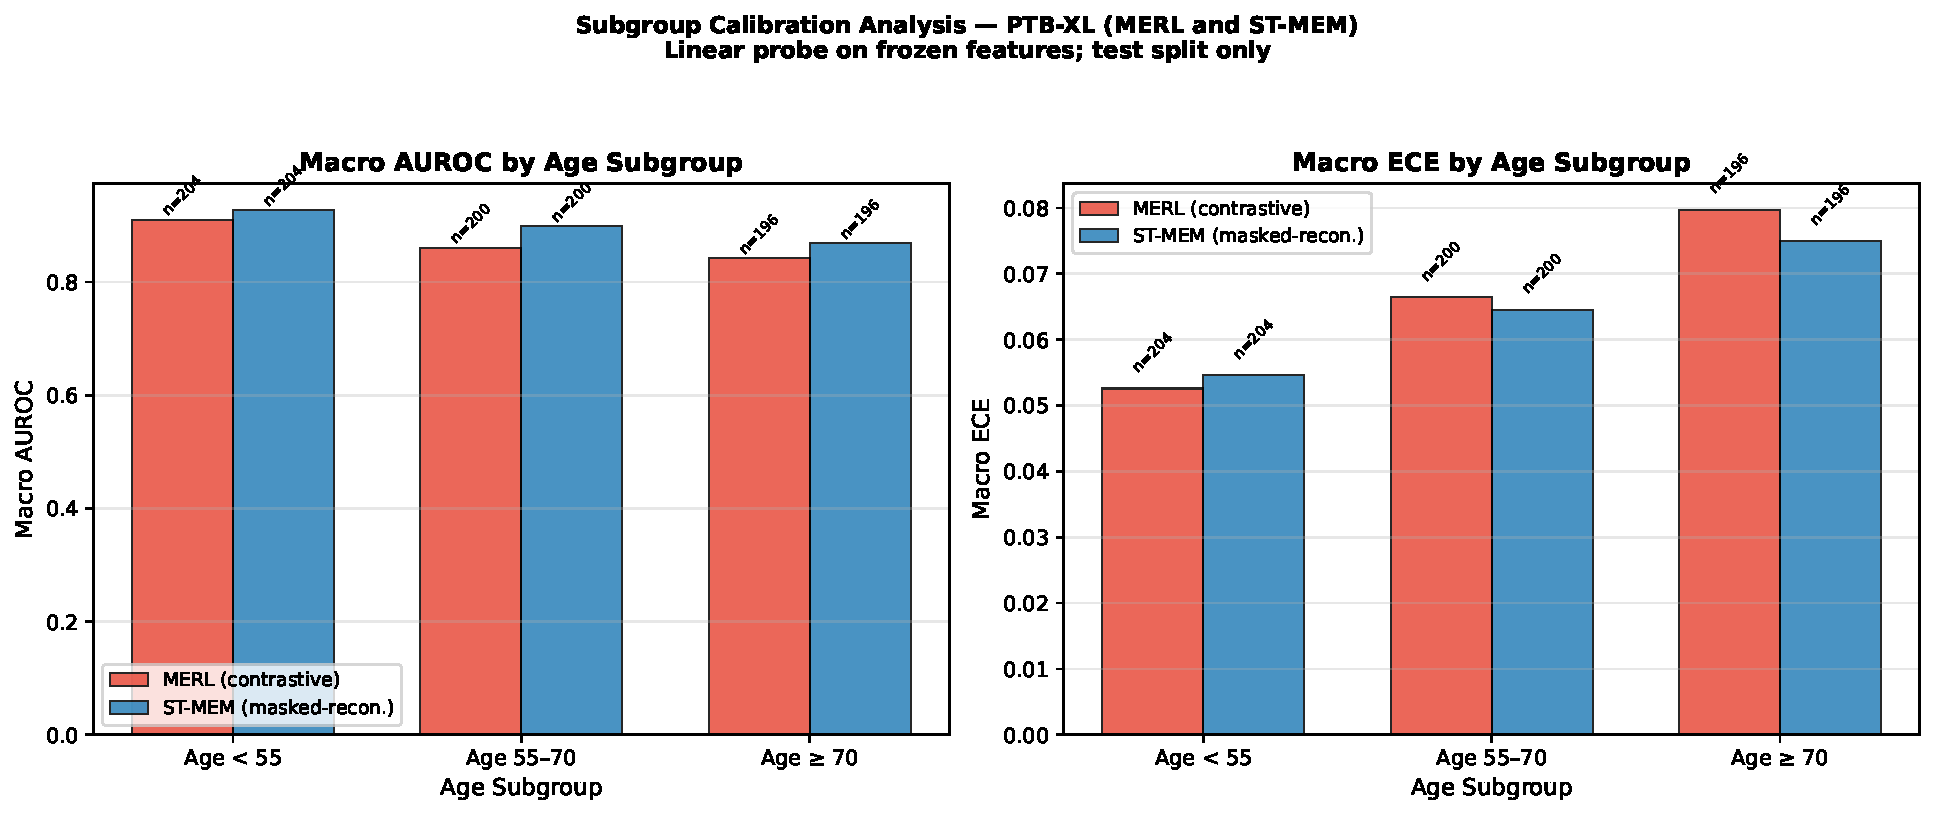
\includegraphics[width=0.95\linewidth]{figures/fig9_subgroup_calibration.pdf}
  \caption{Subgroup AUROC and ECE by age group (PTB-XL test split, linear probe trained on
    70\% of 2{,}000 records). Both models show decreasing AUROC and increasing ECE with age,
    with the largest calibration gap in the $\geq$70 group (MERL ECE 0.080, ST-MEM 0.075).
    \textbf{Note:} this subgroup analysis uses a re-trained probe on a 2{,}000-record sample;
    absolute values differ from the main benchmark.}
  \label{fig:subgroup}
\end{figure}

Both MERL and ST-MEM show a consistent age gradient: ECE increases from age$<$55
(MERL 0.053, ST-MEM 0.055) to age$\geq$70 (MERL 0.080, ST-MEM 0.075), while AUROC decreases
(MERL 0.910$\to$0.842; ST-MEM 0.928$\to$0.869). Sex-based differences are smaller (female
patients show slightly lower ECE). These results use a re-trained probe on the 2{,}000-record
sample, so absolute values differ from Table~\ref{tab:full-benchmark}; the age gradient is
consistent across both models and suggests calibration auditing for elderly populations is
particularly warranted.

\subsection{Cross-Dataset Calibration Transfer}
\label{sec:results-crossdataset}

Figure~\ref{fig:cross-dataset} shows how ECE varies across datasets for each model. The
variation is large: S4D's ECE ranges from 0.010 (CODE-15\%) to 0.064 (PTB-XL), a factor of
${\sim}6\times$; ST-MEM from 0.028 (CODE-15\%) to 0.124 (PTB-XL), ${\sim}4.4\times$; and
HuBERT-ECG from 0.032 to 0.136, ${\sim}4.3\times$. PTB-XL is consistently the hardest to
calibrate and the single-label arrhythmia datasets the easiest, with MIMIC-IV-ECG
intermediate.

\begin{figure}[t]
  \centering
  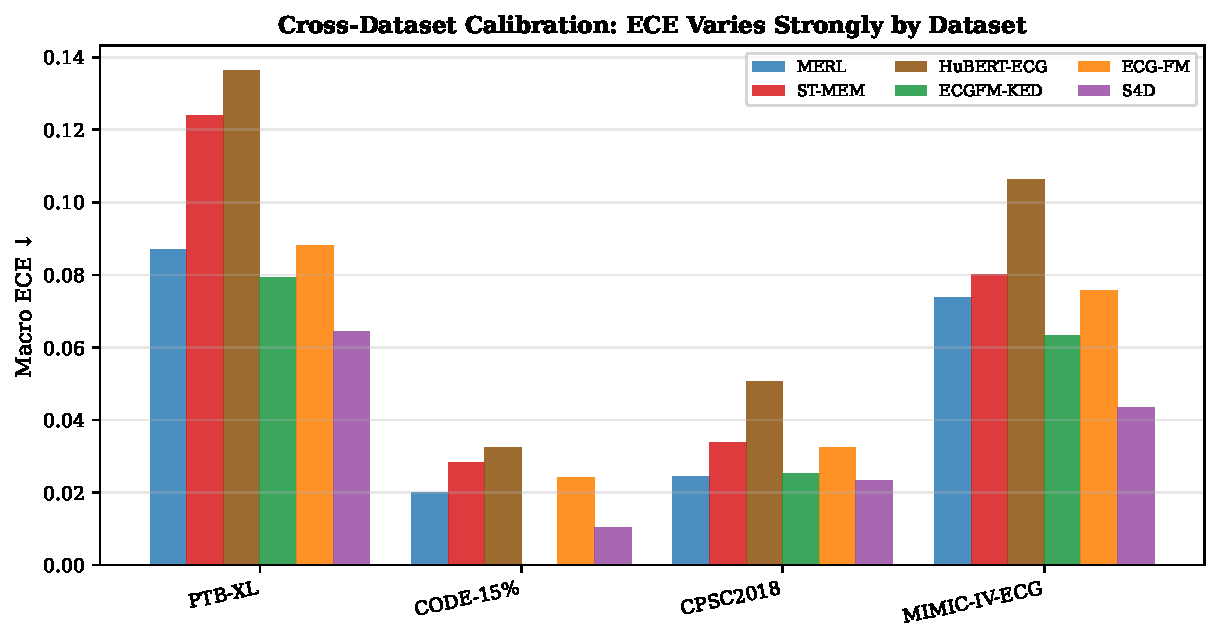
\includegraphics[width=0.98\linewidth]{figures/fig_cross_dataset_ece.pdf}
  \caption{Cross-dataset ECE for all six models. The same model can be well-calibrated on one
    dataset and poorly calibrated on another (up to ${\sim}6\times$ for S4D). Calibration
    audits must therefore be conducted per deployment context.}
  \label{fig:cross-dataset}
\end{figure}

This variation has a direct clinical implication: a calibration audit conducted during
development on one ECG dataset (e.g., CPSC2018 or CODE-15\%) may severely underestimate
miscalibration in production if the deployment population resembles PTB-XL's multi-morbidity
structure. Practitioners should audit calibration on locally representative cohorts before
deployment.

\subsection{Skip Log}
\label{sec:skip-log}

\begin{itemize}
  \item \textbf{HuBERT-ECG (resolved)}: the legacy \texttt{.pth} checkpoint is a non-PyTorch
    binary (unreadable), but the public \texttt{safetensors} checkpoint loads via the
    HuggingFace \texttt{AutoModel} interface. HuBERT-ECG is fully included on all four datasets.
  \item \textbf{MIMIC-IV-ECG (included)}: the 36.3~GB ZIP (800{,}035 records, 1{,}601{,}077
    entries) was validated and staged locally; a 2{,}000-record, natural-prevalence benchmark
    with report-derived labels is included in all analyses. A small number of records with
    NaN lead values were imputed with the per-lead mean before feature extraction.
  \item \textbf{ECGFM-KED $\times$ CODE-15\%}: partial architecture reconstruction (35 missing
    parameter keys); near-chance AUROC. This single cell is excluded from CODE-15\%
    conclusions and the Pareto/composite analyses; ECGFM-KED is retained on the other three
    datasets.
  \item \textbf{LBBB on MIMIC-IV-ECG}: only 9 positive test examples (below the 10-positive
    minimum-support threshold); excluded from MIMIC macro metrics (Table~\ref{tab:mimic-support}).
\end{itemize}
